% Main latex file for the boxcom howto.

% The left footer on the normal pagestyle pages
\newcommand{\normalleftfoot}{This is my stuff}

% The right footer on the normal pagestyle pages
\newcommand{\normalrightfoot}{More stuff}


% The manual_template controls page layout and things like the logo
% in each page footer.
\input{doctools/latex/manual_template.tex}  
\input{doctools/latex/mycommands.tex} % Some useful commands
\input{doctools/latex/units.tex} % Macros for pretty measurement units

% Some text is inserted in drafts that shouldn't be in the released
% version.  For example, some figures have their filenames printed in
% the draft version.  See the \draftnote command in mycommands to
% insert text like this.
\newcommand{\isdraft}{1} % Choose 1 for draft, 0 for release

% isforme
% Choose 1 for in-house use, 0 for outside.  The in-house manual
% will contain the dollar-sign calibration commands
\newcommand{\isforme}{1} % Choose 1 for internal, 0 for outside

% Figure search path
\graphicspath{
              {figs/} % Figures drawn with xfig
              }

% These commands cause  usr_commands.idx and srs_commands.idx to be
% generated when latex is run on this file and the multind.sty file
% is pulled in (by manual_template)
\makeindex{user_cmds_index}
\makeindex{internal_cmds_index}

\begin{document}


%\doublespacing %set double spacing

% Title page
\thispagestyle{empty}   % First page does not need headers and footers
\vspace*{\fill}
\begin{center}
{\huge boxcom howto}\\
\today
\end{center}
\vspace*{\fill}
\clearpage


% Table of contents page
\pagestyle{toc} % Set the toc page style
\tableofcontents{}
\clearpage{}    % There must be a \clearpage to end a page style

\pagestyle{normal} % Set the normal page style

%%%%%%%%%%%%%%%%%%%%%%%%%%%%%%%%%%%%%%%%%%%%%%%%%%%%%%%%%%%%%%%%%%%%%
% The USB board
%
% Subsections:
% 
%%%%%%%%%%%%%%%%%%%%%%%%%%%%%%%%%%%%%%%%%%%%%%%%%%%%%%%%%%%%%%%%%%%%%
\section{USB board}

\subsection{Making connections}
Figure \ref{fig:panel_switch_wiring} shows how the front panel power
switch should be wired.

\begin{figure}[ht]
  \begin{center}
    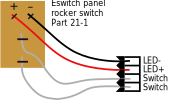
\includegraphics[clip,scale=1]{figs/panel_switch_wiring}
    \caption{Panel switch wiring \label{fig:panel_switch_wiring}}
  \end{center}
\end{figure}

Figure \ref{fig:post_cable} shows how to make the cable connecting the
monitored 3.3V output to the front panel binding posts.
\begin{figure}[ht]
  \begin{center}
    
\includegraphics[clip,scale=1]{figs/post_cable}
    \caption{Panel switch wiring \label{fig:post_cable}}
  \end{center}
\end{figure}


\clearpage{}
\subsection{Board checkout}


\subsubsection{Voltage rails}
Use table \ref{tab:usb_rails} to keep track of voltage rails.

\begin{table}[ht]
  \begin{center}
    \begin{tabular}{|c|c|c|c|}
      \hline
      Net name &Test points &Acceptable &Actual\\
      \hline \hline
      $\mathrm{V_{bus}}$ &TP100 vs.\ TP101 &\cwksentry{1in}{4.5V $\rightarrow$ 5.5V} 
        &\cwksentry{1in}{} \\
      \hline
      $\mathrm{+3.3V_{aux}}$ &TP400 vs.\ TP401 &\cwksentry{1in}{3.14V $\rightarrow$ 3.45V} 
        &\cwksentry{1in}{} \\
      \hline
      $\mathrm{+3.3V_{mon}}$ &TP500 vs.\ TP401 &\cwksentry{1in}{3.14V $\rightarrow$ 3.45V} 
        &\cwksentry{1in}{} \\
      \hline
    \end{tabular}
    \caption{Voltage rail checkout table for the USB
      board.\label{tab:usb_rails}}
  \end{center}
\end{table}

\subsubsection{Current monitor}
The current monitor output at J500 will have a fixed DC output, since
the voltage regulator following it always draws at least 1mA. As
illustrated in figure \ref{fig:monitor_test}, the slope set in
hardware should give $\Delta \mathrm{V_{out}}$ = 1V for each
additional 10mA of current draw from J501.  Since the voltage output
from J501 is controlled at 3.3V, a test load of 3.3k$\Omega$ should
increase the voltage at J500 by 100mV.

\begin{figure}[ht]
  \begin{center}
    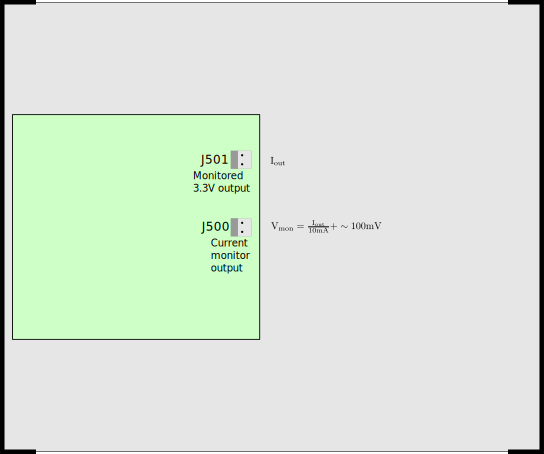
\includegraphics[clip,scale=.5]{figs/monitor_test}
    \caption{The output connectors used during the current monitor test.\label{fig:monitor_test}}
  \end{center}
\end{figure}

\begin{table}[ht]
  \begin{center}
    \begin{tabular}{|c|c|c|}
      \hline
      Load applied to J501 & Acceptable $\mathrm{V_{out}}$ at J500 & Measured $\mathrm{V_{out}}$ at J500\\
      \hline\hline
      Open                 &90mV $\rightarrow$ 110mV &\wksentry{2cm}{$\mathrm{V_{out,o}} =$}\\
      \hline
      3.3k$\Omega$         &\cwksentry{3cm}{$\mathrm{V_{out,o}}$ + 100mV} &\\
      \hline
    \end{tabular}
    \caption{Passing voltage measurements for the current monitor test.\label{tab:monitor_test}}
  \end{center}
\end{table}

\subsubsection{Serial loopback}
The serial loopback test is a basic test of the USB/serial interface
and the RS-232 transceiver.  Make the breakout cable shown in figure
\ref{fig:db9_breakout}, then make connections to the board as shown in
figure \ref{fig:serial_loopback}.

\begin{figure}[ht]
  \begin{center}
    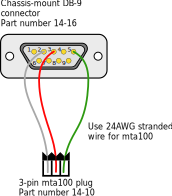
\includegraphics[clip,scale=1]{figs/usb_board_uart_to_db9}
    \caption{Wiring the DB9 breakout cable for the serial loopback
      test.\label{fig:db9_breakout}}
  \end{center}
\end{figure}

\begin{figure}[ht]
  \begin{center}
    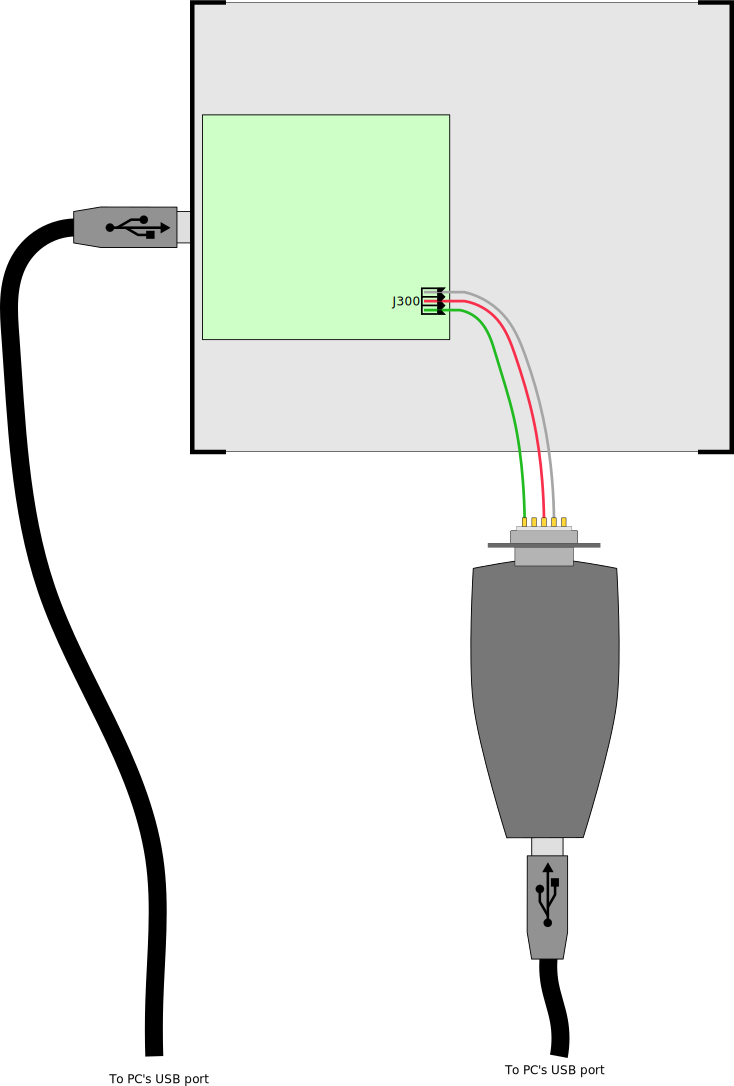
\includegraphics[clip,scale=0.5]{figs/serial_loopback_test}
    \caption{The setup for the serial loopback
      test.\label{fig:serial_loopback}}
  \end{center}
\end{figure}

The serial loopback test script is:
\begin{center}
  \texttt{boxcom/implement/data/scripts/tty\_loopback.py}
\end{center}
...and the test should pass at the speed listed in table
\ref{tab:loopback_test}.

\begin{table}[ht]
  \begin{center}
    \begin{tabular}{|c|c|}\hline
      Minimum passing baud  &Measured passing baud\\
      \hline\hline
      \cwksentry{5cm}{115200} &\cwksentry{5cm}{}\\
      \hline
    \end{tabular}
    \caption{Passing baud measurement for the serial loopback test.
      The usb board should be able to reliably pass the loopback test
      for data flowing in both directions at the minimum
      baud.\label{tab:loopback_test}}
  \end{center}
\end{table}

\clearpage{}
\subsection{Schematics}

% Control top-bottom placement with the vspace parameter
\begin{figure}[ht]
    \begin{center}
          \vspace{0.4cm}
          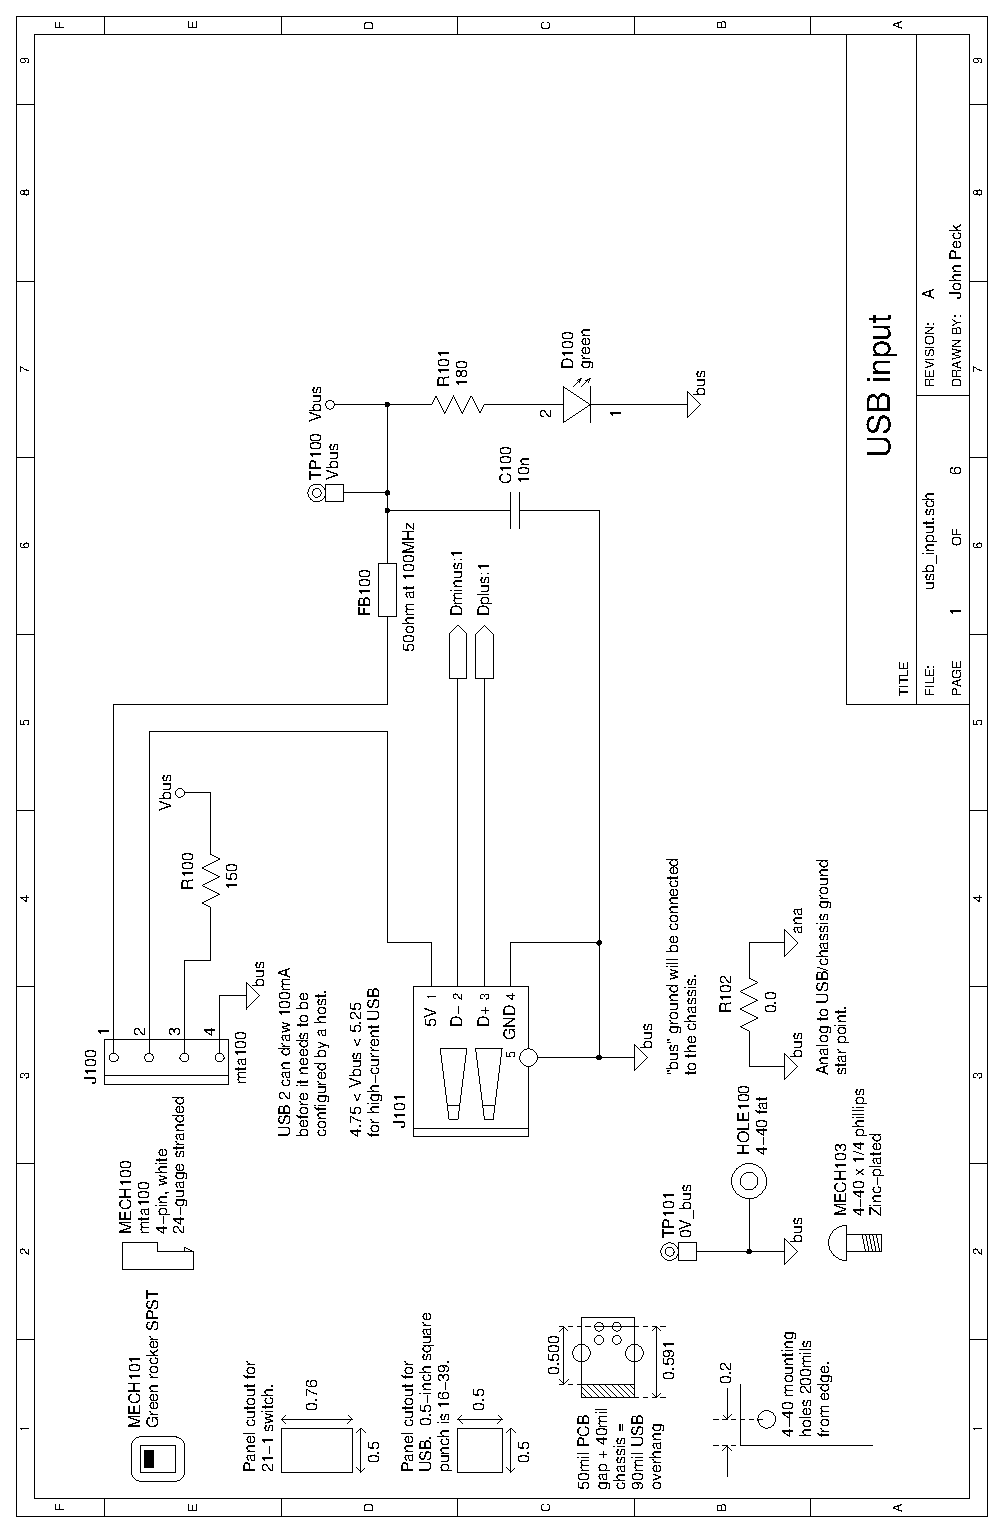
\includegraphics[clip,height=\textheight]
          {schematics/usb/usb_input}
          \label{sch:usb_input}
    \end{center} 
\end{figure}

\begin{figure}[ht]
    \begin{center}
          \vspace{0.4cm}
          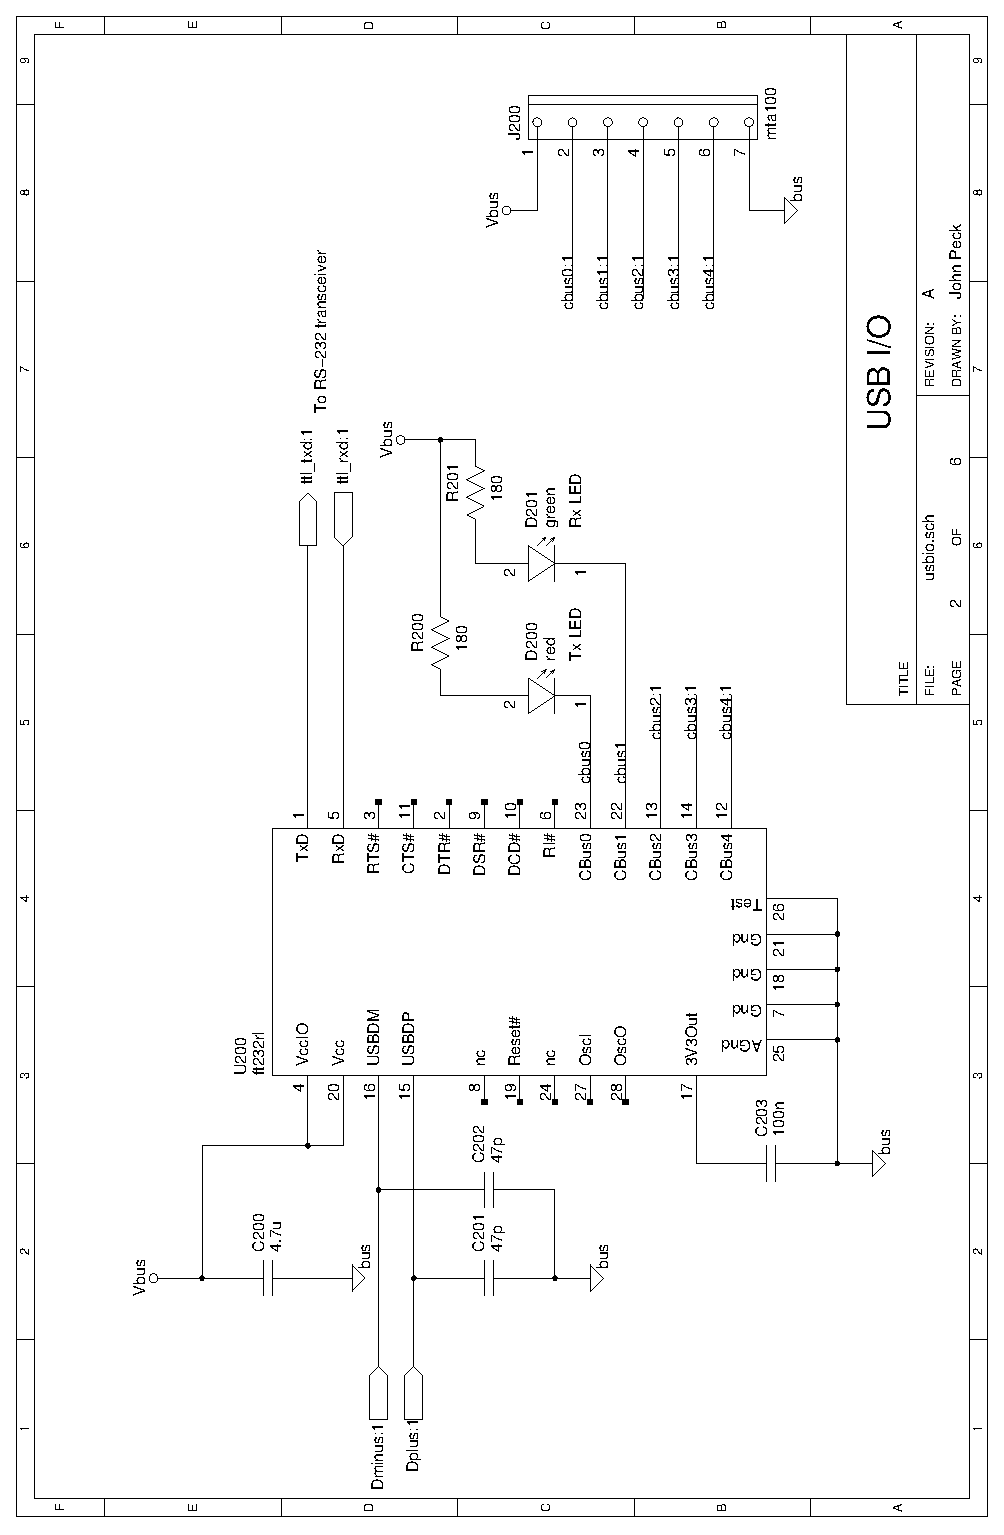
\includegraphics[clip,height=\textheight]
          {schematics/usb/usbio}
          \label{sch:usbio}
    \end{center} 
\end{figure}

\begin{figure}[ht]
    \begin{center}
          \vspace{0.4cm}
          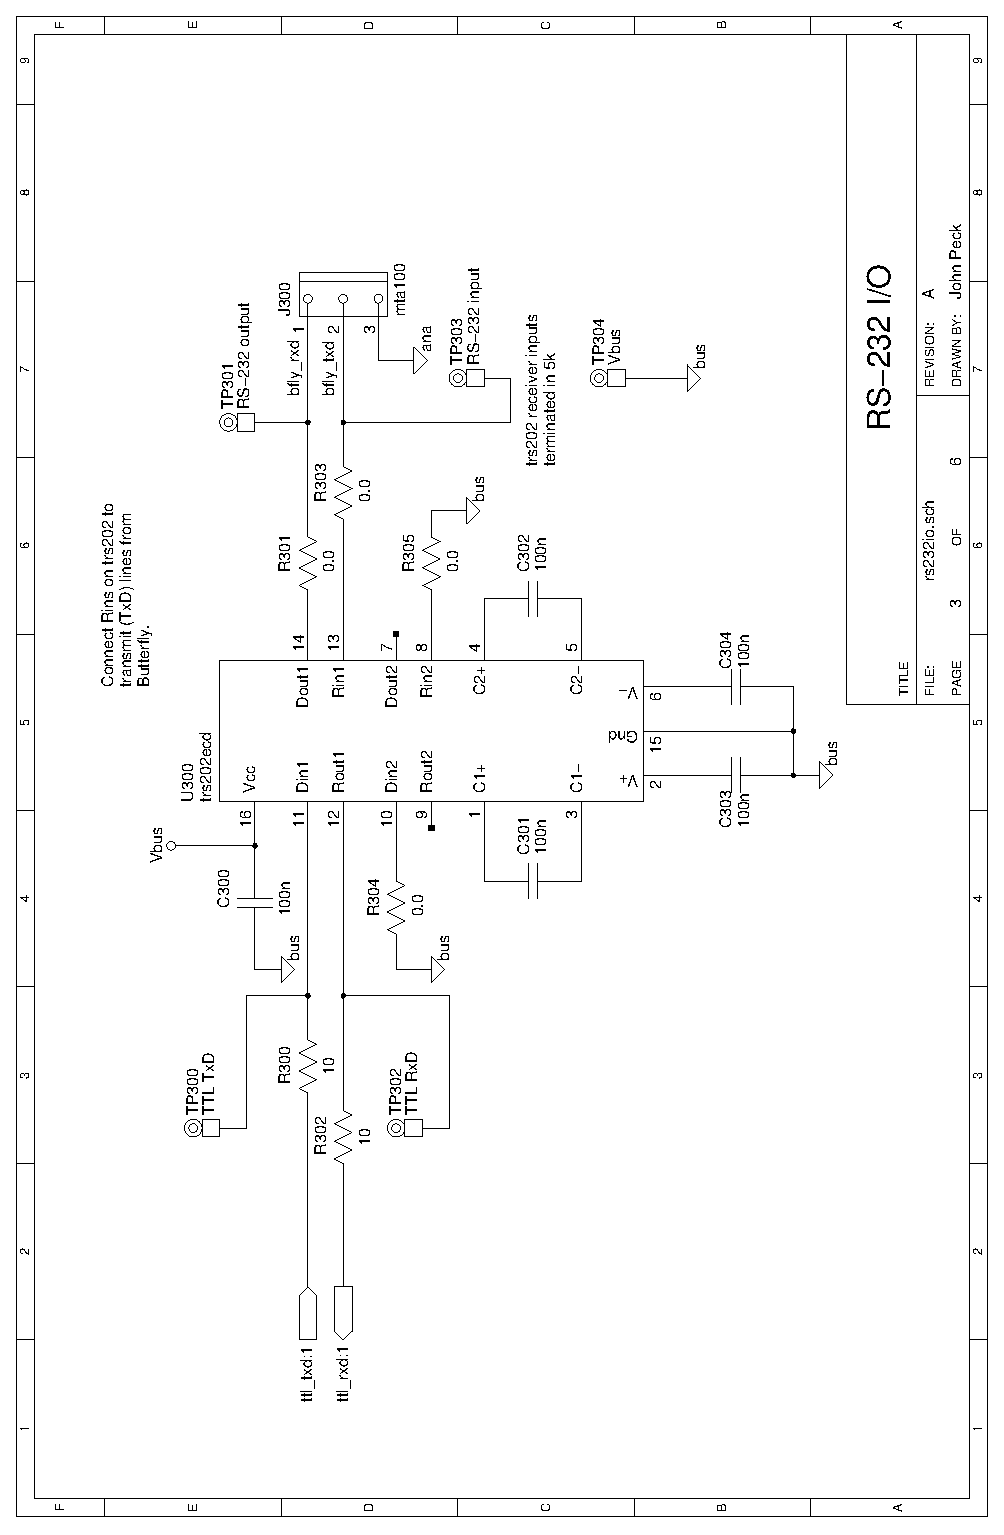
\includegraphics[clip,height=\textheight]
          {schematics/usb/rs232io}
          \label{sch:rs232io}
    \end{center} 
\end{figure}

\begin{figure}[ht]
    \begin{center}
          \vspace{0.4cm}
          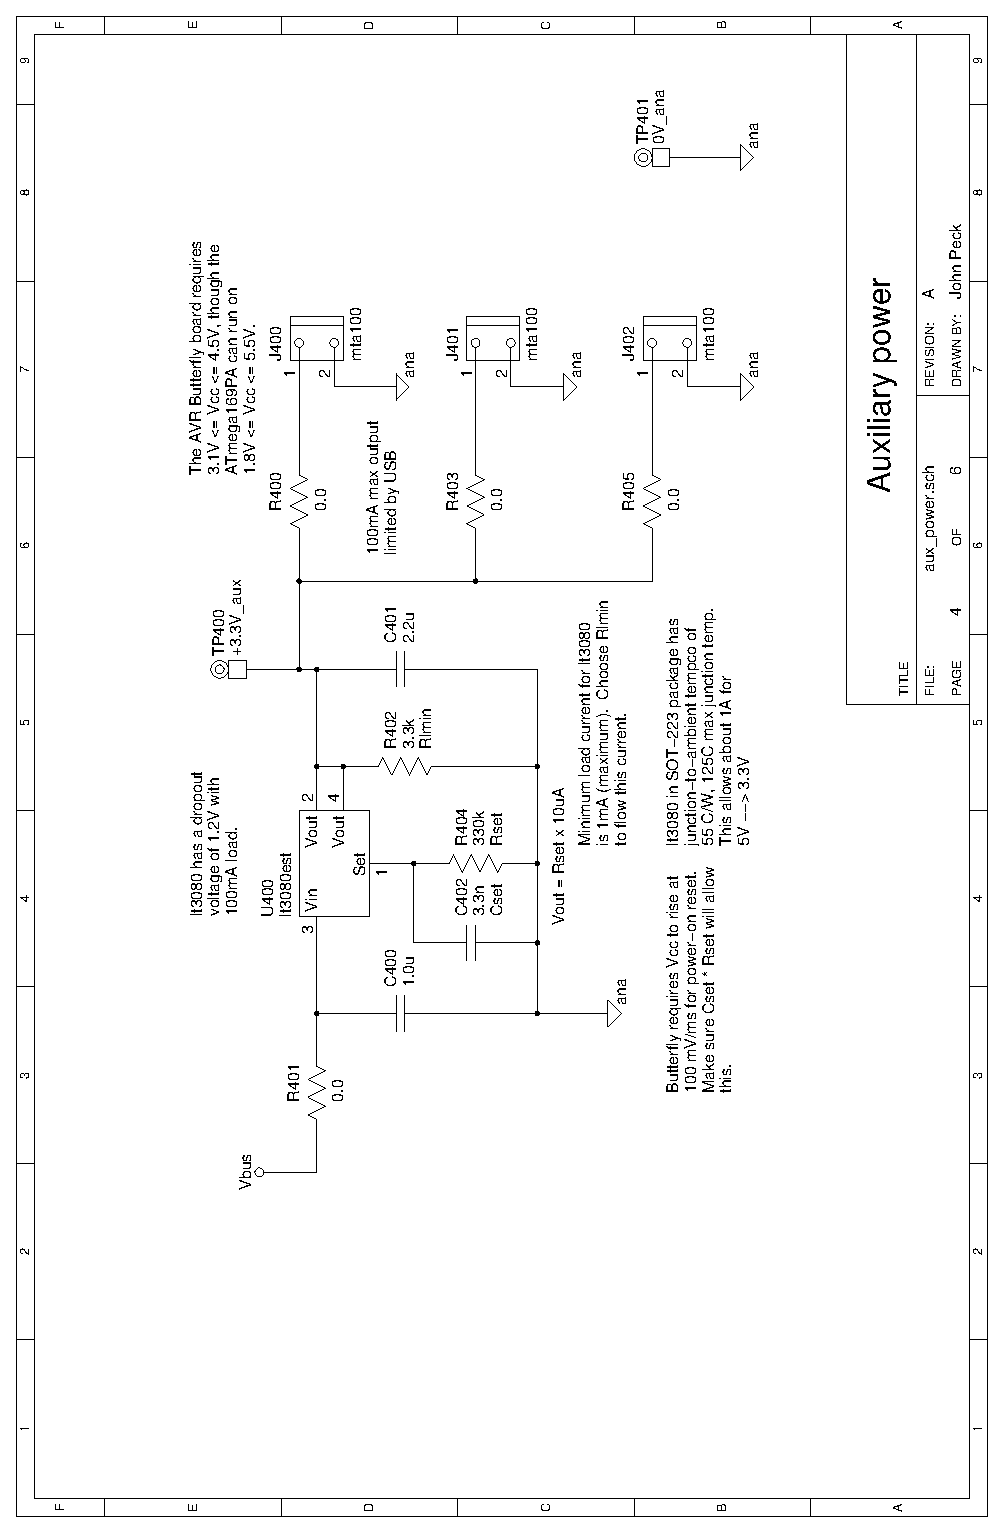
\includegraphics[clip,height=\textheight]
          {schematics/usb/aux_power}
          \label{sch:aux_power}
    \end{center} 
\end{figure}

\begin{figure}[ht]
    \begin{center}
          \vspace{0.4cm}
          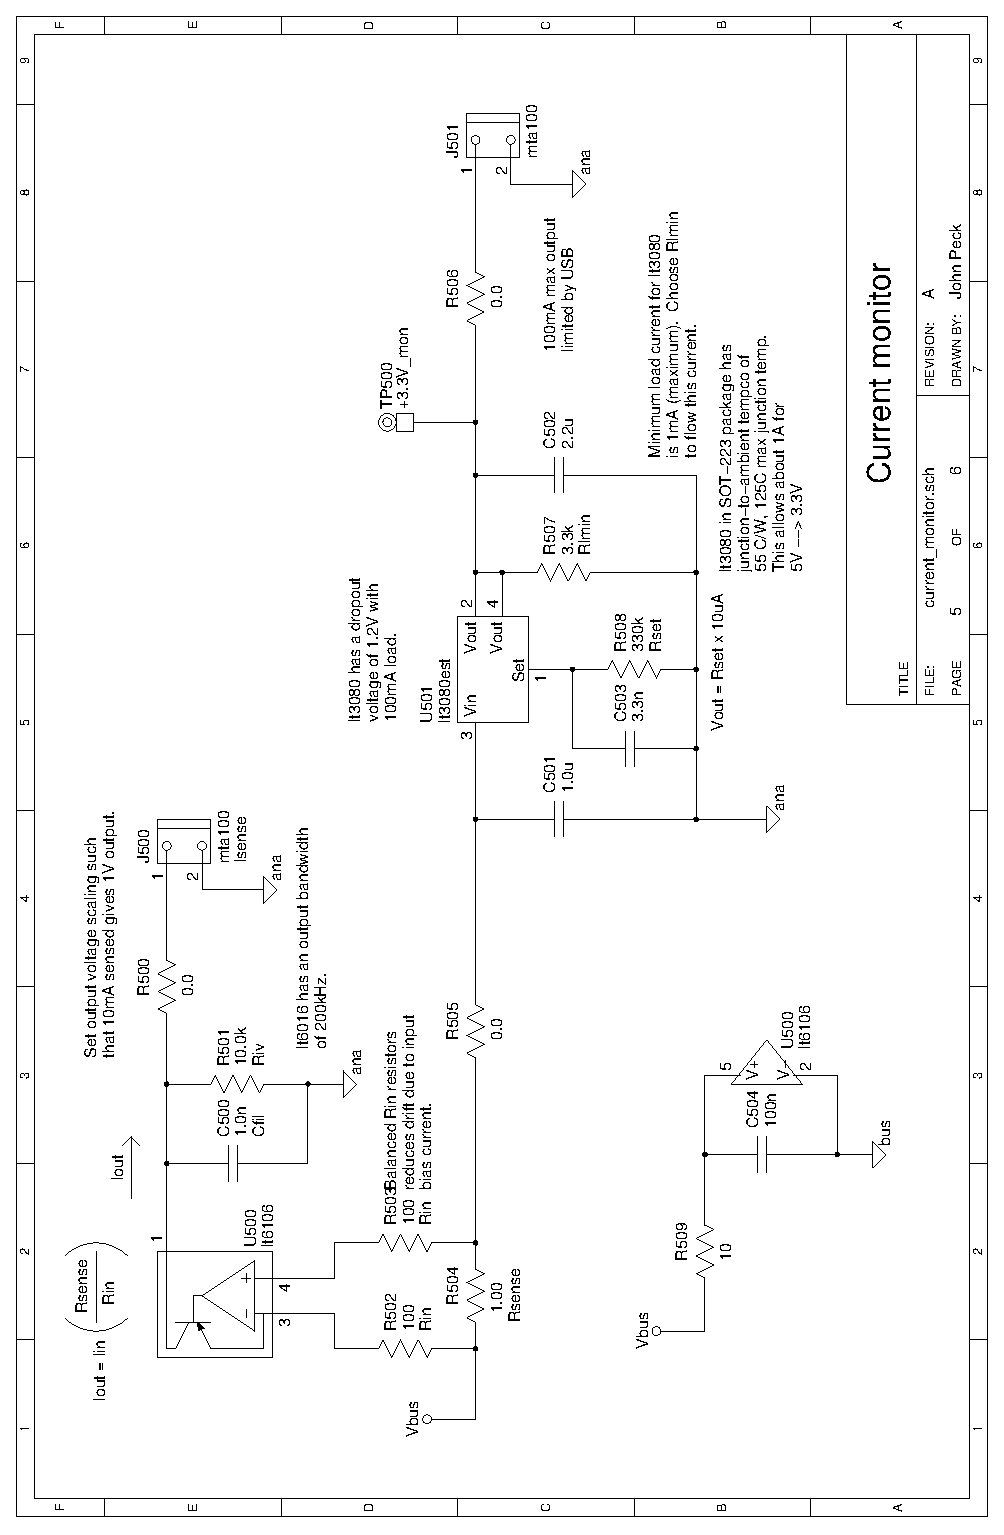
\includegraphics[clip,height=\textheight]
          {schematics/usb/current_monitor}
          \label{sch:current_monitor}
    \end{center} 
\end{figure}

\begin{figure}[ht]
    \begin{center}
          \vspace{0.4cm}
          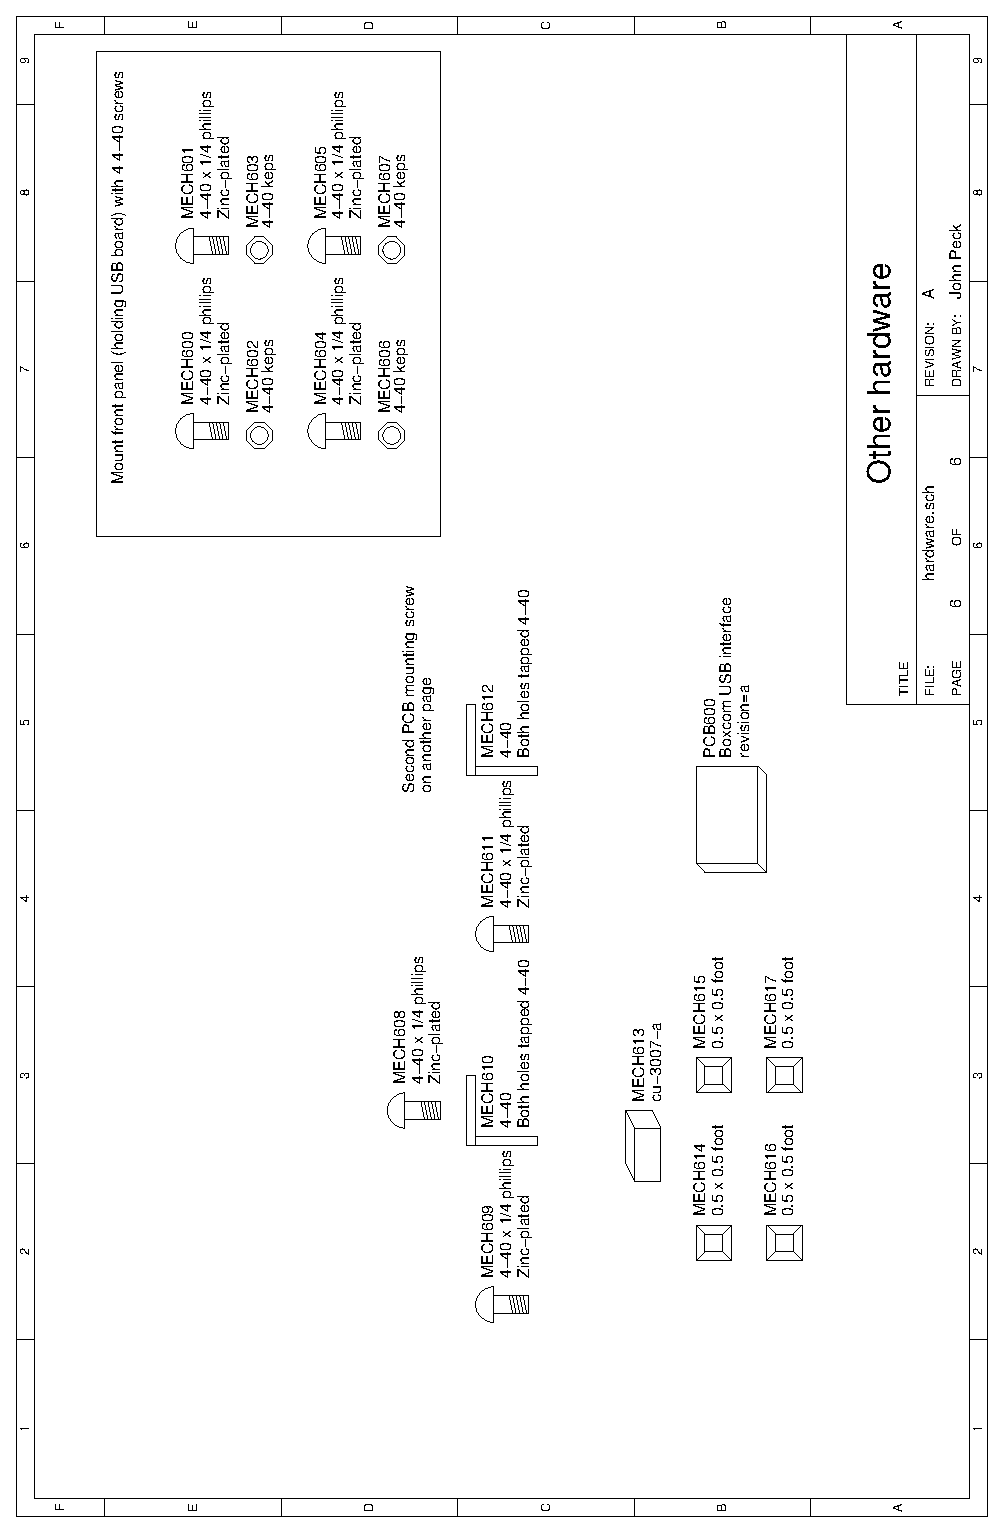
\includegraphics[clip,height=\textheight]
          {schematics/usb/hardware}
          \label{sch:hardware}
    \end{center} 
\end{figure}

%%%%%%%%%%%%%%%%%%%%%%%%%%%%%%%%%%%%%%%%%%%%%%%%%%%%%%%%%%%%%%%%%%%%%
% The Butterfly board
%
% Subsections:
% 
%%%%%%%%%%%%%%%%%%%%%%%%%%%%%%%%%%%%%%%%%%%%%%%%%%%%%%%%%%%%%%%%%%%%%
\section{Butterfly board}

\subsection{Making connections}
Figure \ref{fig:bfly_connect} shows the connections that should be made to
the Butterfly board.

\begin{figure}[ht]
  \begin{center}
    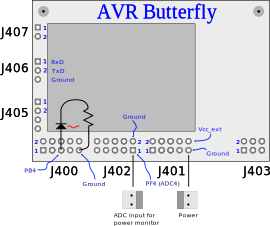
\includegraphics[clip,scale=1]{figs/butterfly_connect}
    \caption{Connections to the AVR Butterfly \label{fig:bfly_connect}}
  \end{center}
\end{figure}

Figure \ref{fig:uart_cable} shows how the UART cable should be made.
\begin{figure}[ht]
  \begin{center}
    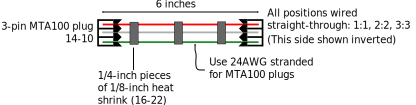
\includegraphics[clip,scale=1]{figs/uart_cable}
    \caption{The UART cable connecting the Butterfly and USB
      boards.\label{fig:uart_cable}}
  \end{center}
\end{figure}

Figure \ref{fig:bfly_power_cable} shows how to make the power cable.
\begin{figure}[ht]
  \begin{center}
    
\includegraphics[clip,scale=1]{figs/butterfly_power_cable}
    \caption{The power cable connecting the Butterfly and the USB
      boards.  The cable should run from J400 on the USB board to the
      power connector shown in figure
      \ref{fig:bfly_connect}.\label{fig:bfly_power_cable} }
  \end{center}
\end{figure}

Figure \ref{fig:isense_cable} shows how to make the cable connecting
the USB board's current sense output to the Butterfly's ADC input.
\begin{figure}[ht]
  \begin{center}
    
\includegraphics[clip,scale=1]{figs/current_sense_cable}
    \caption{The cable connecting the Butterfly board's power monitor
      input to the USB board's output.\label{fig:isense_cable} }
  \end{center}
\end{figure}




%%%%%%%%%%%%%%%%%%%%%%%%%%%%%%%%%%%%%%%%%%%%%%%%%%%%%%%%%%%%%%%%%%%%%
% Firmware
%
% Subsections:
% 
%%%%%%%%%%%%%%%%%%%%%%%%%%%%%%%%%%%%%%%%%%%%%%%%%%%%%%%%%%%%%%%%%%%%%
\section{Firmware}


\subsection{Adding a new remote command}
\newcounter{comcount}

\setcounter{comcount}{1}
\paragraph{\arabic{comcount} --  Choose a name for the command}
The command characters, the argument characters, one space, and one
string terminator must all fit in the received command buffer. The
definition of this size is shown below.

\filesnip{bx\_command.h}
{ \texttt{\#define RECEIVE\_BUFFER\_SIZE 20} }

\addtocounter{comcount}{1}
\paragraph{\arabic{comcount} -- Think about the command's arguments}
The code can only handle unsigned hexadecimal number arguments
formatted as strings.  If you need something else, you'll have to
write more code.

\addtocounter{comcount}{1}
\paragraph{\arabic{comcount} -- Add a function for your command to call}
I like to put the new function in the module where it belongs, and
just add a ``cmd\_'' prefix to it.  If the command is a query, I add a
``\_q'' suffix.  The command corresponding to the \texttt{vcounts?}
query is shown below.

\begin{center}
  \vspace{-\baselineskip}
  \begin{tabular}{|l|} \hline
    \rowcolor[gray]{0.8}
    \begin{minipage}[c]{\textwidth - 2\tabcolsep}
      \textbf{File:}
      bx\_adc.c
    \end{minipage}\\
    \begin{minipage}[c]{\textwidth - 2\tabcolsep}
      \vspace{0.5\baselineskip}
      $\cdots$ \\
      \begin{minipage}[c]{\textwidth - 2\tabcolsep}
        \lstset{language=c}
        \begin{lstlisting}
void cmd_vcounts_q(uint16_t nonval) {
  uint16_t adc_temp = 0;
  adc_temp = adc_read();
  usart_printf_p(PSTR("0x%x\r\n"),adc_temp);
}
        \end{lstlisting}
      \end{minipage}
      $\cdots$\\
      \vspace{-0.5\baselineskip}
    \end{minipage}\\
    \hline
  \end{tabular}
\end{center}


\addtocounter{comcount}{1}
\paragraph{\arabic{comcount} -- Give the new command an entry in the command array}
A sample entry in the command array is shown below.  New entries must
be added before the ``end of table indicator.'' Remember that
hexadecimal arguments larger than 4 characters don't make sense for
16-bit integers (leading \texttt{0x} characters are not allowed).

\begin{center}
  \vspace{-\baselineskip}
  \begin{tabular}{|l|} \hline
    \rowcolor[gray]{0.8}
    \begin{minipage}[c]{\textwidth - 2\tabcolsep}
      \textbf{File:}
      bx\_command.c
    \end{minipage}\\
    \begin{minipage}[c]{\textwidth - 2\tabcolsep}
      \vspace{0.5\baselineskip}
      $\cdots$ \\
      \begin{minipage}[c]{\textwidth - 2\tabcolsep}
        \lstset{language=c}
        \begin{lstlisting}
command_t command_array[] ={
  // hello -- Print a greeting.
  {"hello",           // Name of the command
    "none",            // Argument type (can be "none" or "hex" right now)
    0,                 // Maximum number of characters in argument
    &cmd_hello,        // Address of function to execute
    helpstr_hello},    // The help text (defined above)  
  // End of table indicator.  Must be last.
  {"","",0,0,nullstr}
};      
\end{lstlisting}
      \end{minipage}
      $\cdots$\\
      \vspace{-0.5\baselineskip}
    \end{minipage}\\
    \hline
  \end{tabular}
\end{center}


\clearpage
\subsection{Logger functions}

% logger_msg_p
\subsubsection{\texttt{logger\_msg\_p}}
\onecodeline{void logger_msg_p( char *logsys,
  logger_level_t loglevel, const char *logmsg, ... );
}
\textsl{Send a message to the logger module from permanent memory}  


\paragraph{Parameters}
\begin{itemize}
\item \texttt{logsys}
  \subitem Pointer to a string matching one of the logger system strings.
\item \texttt{loglevel}
  \subitem One of the logger level identifiers:
  \subsubitem \verb8log_level_ISR8 (lowest level)
  \subsubitem \verb8log_level_INFO8
  \subsubitem \verb8log_level_WARNING8
  \subsubitem \verb8log_level_ERROR8 (highest level)
\item \texttt{logmsg} \subitem Pointer to a string stored in
  permanent (flash) memory.  This might be a C format string.
\item \texttt{...} \textsl{(additional arguments)} 
  \subitem Depending on the format string, the function may expect a
  sequence of additional arguments, each containing a value to be used
  to replace a format specifier in the format string.  There should be
  at least as many of these arguments as the number of values
  specified in the format specifiers. Additional arguments are ignored
  by the function.
\end{itemize}

\paragraph{Examples}

\begin{center}
  \begin{minipage}[c]{\textwidth}
    \lstset{language=c,backgroundcolor=\color{codegray},
      showstringspaces=false,breaklines=false}
    \begin{lstlisting}
 logger_msg_p("command",log_level_INFO,
	      PSTR("Command '%s' recognized.\r\n"),command_array -> name);
    \end{lstlisting}
  \end{minipage}
\end{center}
Output (After receiving the \texttt{hello} command):
\boxcmd{[I](command) Command 'hello' recognized.}




%--------------------------------------------------------------------
% Bibliography
%
% 
%--------------------------------------------------------------------
\clearpage
% \addcontentsline{toc}{section}{Bibliography}
% \pagestyle{references} %set the references page style
% \bibliography{doctools/latex/ecrefs.bib}

















%%%%%%%%%%%%%%%%%%%%%%%%%%%%%%%%%%%%%%%%%%%%%%%%%%%%%%%%%%%%%%%%%%%%%%%%%%%
%Everything below here goes in the appendix
%%%%%%%%%%%%%%%%%%%%%%%%%%%%%%%%%%%%%%%%%%%%%%%%%%%%%%%%%%%%%%%%%%%%%%%%%%%
\appendix





%%%%%%%%%%%%%%%%%%%%%%%%%%%%%%%%%%%%%%%%%%%%%%%%%%%%%%%%%%%%%%%%%%%%%%%%%%%
% Indexes
%
%
%%%%%%%%%%%%%%%%%%%%%%%%%%%%%%%%%%%%%%%%%%%%%%%%%%%%%%%%%%%%%%%%%%%%%%%%%%%




% Redefine the printindex command to format the index in multiple columns.
% Uses the multicol package.  
% Don't try to use column separators (lines) -- there's still something
% strange going on with column widths.
%
% printindex still takes two arguments:
% 1. The ind file containing the index entries
% 2. The name for the index (will appear in the table of contents and at the
%    top of the index page.
\renewcommand{\printindex}[2]{
  % The \endtheindex command redefined by multind confounds the multicol
  % environment.  Redefine it to do nothing.  
  \renewcommand{\endtheindex}{}
  \addcontentsline{toc}{section}{#2}
  % Ideally, printindex would take an argument for the number of columns
  % instead of just hard coding it.
  \begin{multicols}{4}
    [\section*{#2}]
    \input{#1.ind}
  \end{multicols}
}% end printindex





% Alphabetical command index
\printindex{user_cmds_index}{Alphabetical command index}

%Internal SRS commands
\ifthenelse{\equal{\isforme}{1}}{
\clearpage{}
\printindex{internal_cmds_index}{Internal command index}
}{}



\end{document}
